\documentclass[dvipsnames,tikz]{standalone}
\usepackage{amsmath}
\usepackage{xcolor}
\usepackage{tikz}
\usepackage{cmbright}      % sansfont
\usetikzlibrary{calc}
\usetikzlibrary{decorations.pathreplacing,calligraphy,3d}


\begin{document}
	% add color=white for dark mode
	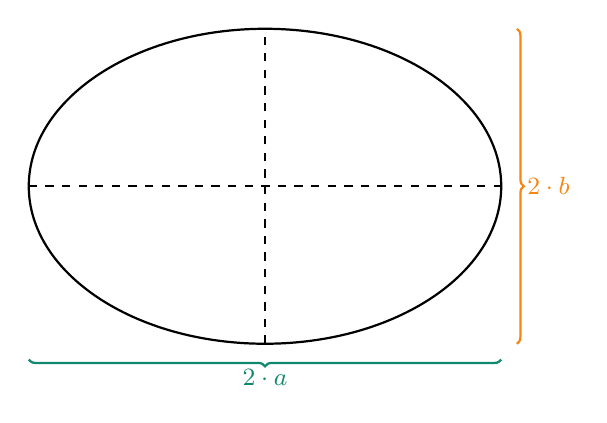
\begin{tikzpicture}[thick, color=black] 

		\draw (0,0) ellipse (3cm and 2cm);
		\draw[dashed] (-3,0) -- (3,0);
		\draw[dashed] (0,-2) -- (0,2);
		
		\begin{scope}[font=\small]
			\draw [PineGreen, decoration={brace,mirror},decorate] (-3,-2.2) -- (3,-2.2) node [pos=0.5, below] {$2\cdot a$}; 
			\draw [BurntOrange, decoration={brace,mirror},decorate] (3.2,-2) -- (3.2,2) node [pos=0.5, right] {$2\cdot b$}; 
		\end{scope}
	\end{tikzpicture} 
	
\end{document}